\chapter*{Funciones trigonométricas}
\setcounter{chapter}{1}
\setcounter{section}{0}

\section{Radianes}
\blueBox{Definición}{
    Un ángulo cualquiera $\alpha$ y la circunferencia de radio $1$ con centro el vértice de $\alpha$, se llaman \emph{radianes} a la longitud del arco que forma el ángulo $\alpha$ con la circunferencia.
}

\begin{center}
    \includegraphics[width=0.8\linewidth]{func_trig1.jpg}
\end{center}

$$360^\circ = 2 \pi rad \Rightarrow 1 rad = \left(\frac{180}{\pi}\right)^\circ \approx 57,3^\circ$$

\begin{center}
    \begin{tabular}{c|c}
        \textbf{Grados} & \textbf{Radianes} \\
        \hline \hline
        $360^\circ$ & $2 \pi rad$ \\
        \hline
        $180^\circ$ & $\pi rad$ \\
        \hline
        $90^\circ$ & $\frac{\pi}{2} rad$ \\
        \hline
        $60^\circ$ & $\frac{\pi}{3} rad$ \\
        \hline
        $45^\circ$ & $\frac{\pi}{4} rad$ \\
        \hline
        $30^\circ$ & $\frac{\pi}{6} rad$ \\
        \hline
        $57,3^\circ$ & $1 rad$ \\
        \hline
        $0^\circ$ & $0 rad$ \\
    \end{tabular}
\end{center}

\section{Funciones periódicas}
\blueBox{Definición}{
    Decimos que una función $f$ es \emph{periódica} con \emph{período T}, si para toda \emph{x} del dominio de $f$, se verifica que $x + T$ también pertenece al dominio de $f$ y además
    $$f(x) = f(x + T)$$

    \tcblower{\textbf{Ejemplo: }}{
        Las funciones $f(x) = \sin(x)$ y $g(x) = \cos(x)$ son periódicas con período $2 \pi$.
    }
}

\section{Gráficas de Seno, Coseno y Tangente}

$$Seno:$$
\begin{center}
    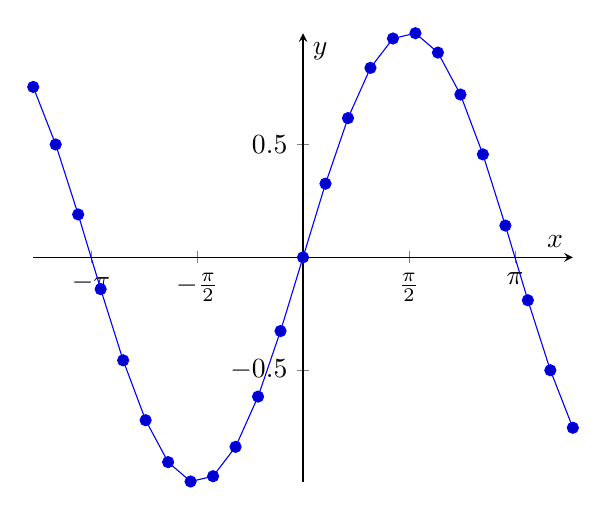
\begin{tikzpicture}
        % sin graph
        \begin{axis}[
            axis x line = center,
            axis y line = center,
            domain=-4:4,legend pos=outer north east,
            xlabel=$x$,ylabel=$y$,
            xtick={
                -6.28318, -4.7123889, -3.14159, -1.5708,
                1.5708, 3.14159, 4.7123889, 6.28318
            },
            xticklabels={
                $-2\pi$, $-\frac{3\pi}{2}$, $-\pi$, $-\frac{\pi}{2}$,
                $\frac{\pi}{2}$, $\pi$, $\frac{3\pi}{2}$, $2\pi$
            }
            ]
            \addplot {sin(deg(x))}; 
        \end{axis}
    \end{tikzpicture}
\end{center}
$$C_0 = \{ k \pi / k \in \Z \}$$
$$Coseno:$$
\begin{center}    
    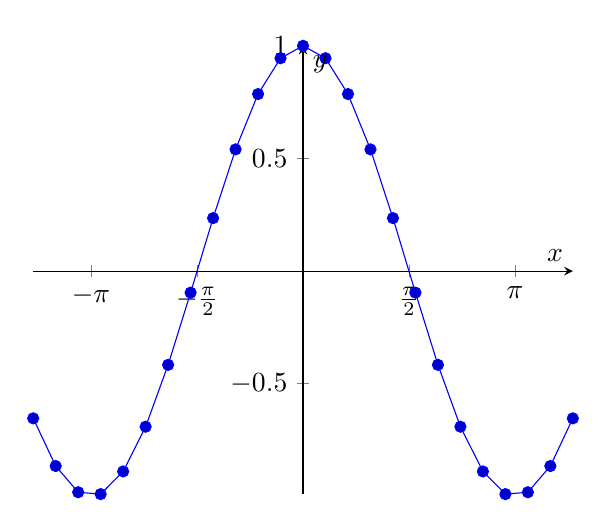
\begin{tikzpicture}
        % sin graph
        \begin{axis}[
            axis x line = center,
            axis y line = center,
            domain=-4:4,legend pos=outer north east,
            xlabel=$x$,ylabel=$y$,
            xtick={
                -6.28318, -4.7123889, -3.14159, -1.5708,
                1.5708, 3.14159, 4.7123889, 6.28318
            },
            xticklabels={
                $-2\pi$, $-\frac{3\pi}{2}$, $-\pi$, $-\frac{\pi}{2}$,
                $\frac{\pi}{2}$, $\pi$, $\frac{3\pi}{2}$, $2\pi$
            }
            ]
            \addplot {cos(deg(x))}; 
        \end{axis}
    \end{tikzpicture}
\end{center}
$$C_0 = \{ (2k + 1) \frac{\pi}{2} / k \in \Z \}$$
$$Tangente:$$
\begin{center}    
    \includegraphics[width=0.8\linewidth]{func_tan.jpg}
\end{center}
$$C_0 = \{ k\pi / k \in \Z \}$$

\section{Función Sinusoidal}
\blueBox{Definición}{
    La función \emph{sinusoidal} es toda función que cumpla:
    $$f: \R \rightarrow \R / f(x) = a \sin(bx+c)$$
    donde $a,b,c \in \R$ y además $a \neq 0$ y $b \neq 0$
}

Si cambiamos el valor de $a$, cambiamos la \textbf{amplitud} de la función, que cambia el valor máximo y mínimo de la función.

\begin{center}
    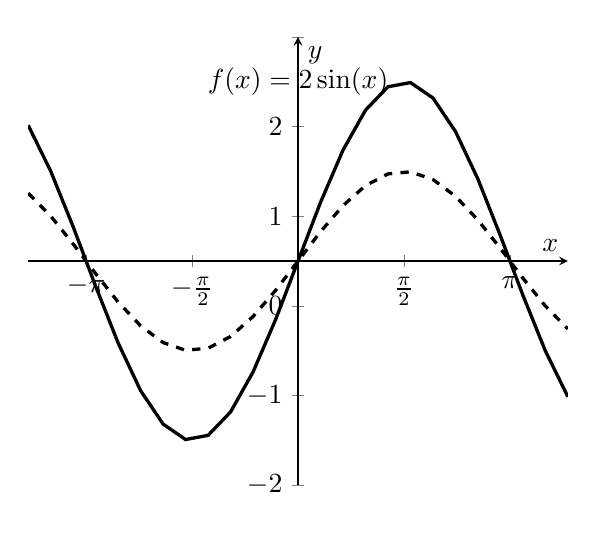
\begin{tikzpicture}
        \begin{axis}[
            axis x line = center,
            axis y line = center,
            domain=-4:4,legend pos=outer north east,
            ymin=-2.5,ymax=2.5,
            xlabel=$x$,ylabel=$y$,
            xtick={
                -6.28318, -4.7123889, -3.14159, -1.5708,
                1.5708, 3.14159, 4.7123889, 6.28318
            },
            xticklabels={
                $-2\pi$, $-\frac{3\pi}{2}$, $-\pi$, $-\frac{\pi}{2}$,
                $\frac{\pi}{2}$, $\pi$, $\frac{3\pi}{2}$, $2\pi$
            },
            ytick={
                -2.5, -1.5, -0.5, 0.5, 1.5, 2.5
            },
            yticklabels={
                $-2$, $-1$, $0$, $1$, $2$
            }
            ]
            \addplot [color=black, very thick, dashed]{sin(deg(x))};
            \addplot [color=black, very thick]{2*sin(deg(x))};
            \node at (axis cs:0,2) {$f(x) = 2 \sin(x)$};
        \end{axis}
    \end{tikzpicture}
\end{center}

Si cambiamos el valor de $b$, cambiamos la \textbf{período} de la función, que cambia la cantidad de veces que se repite la función en un intervalo.
$$T = \frac{2\pi}{|b|}$$

\begin{center}
    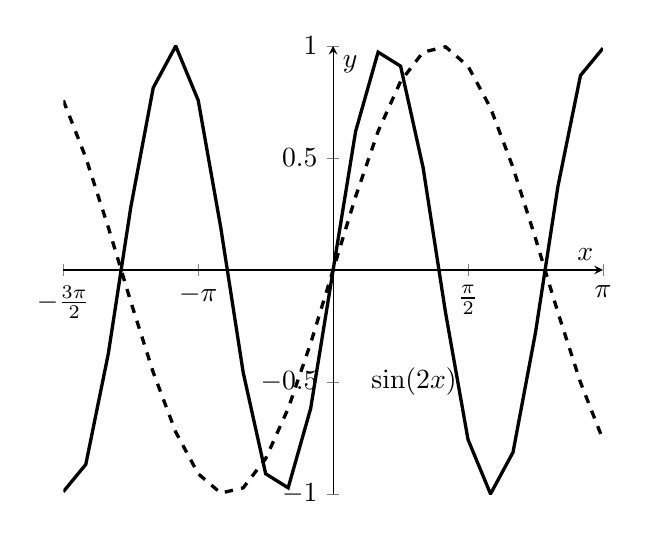
\begin{tikzpicture}
        \begin{axis}[
            axis x line = center,
            axis y line = center,
            domain=-4:4,legend pos=outer north east,
            ymin=-1,ymax=1,
            xlabel=$x$,ylabel=$y$,
            xticklabels={
                $-2\pi$, $-\frac{3\pi}{2}$, $-\pi$, $-\frac{\pi}{2}$,
                $\frac{\pi}{2}$, $\pi$, $\frac{3\pi}{2}$, $2\pi$
            }
            ]
            \addplot [color=black, very thick, dashed]{sin(deg(x))};
            \addplot [color=black, very thick]{sin(2*deg(x))};
            \node at (axis cs:1.2,-0.5) {$\sin(2x)$};
        \end{axis}
    \end{tikzpicture}
\end{center}

Por último, el número $c$ se conoce como \emph{fase inicial} de la función\\
Considerando la función:
$$f: \R \rightarrow \R / f(x) = a \sin(bx+c)$$ 
supongamos que $a > 0$. Para graficarla podemos seguir los siguientes pasos
\begin{enumerate}
    \item Su amplitud, $a$, nos indica el valor máximo y mínimo de la función. Por lo tanto, el eje $y$ se extiende desde $-a$ hasta $a$.
    \item $f(x) = 0 \Leftrightarrow bx+c = 0 \Leftrightarrow x = -\frac{c}{b}$. Este valor, $x_i$, es el "inicio" de la onda.
    \item Calculamos el período $T = \frac{2\pi}{|b|}$ y determinamos el "final" de la onda: $x_f = x_i + T$ (una onda "termina" donde "empiza la siguiente").\\
    Estos cuatro números $a, -a, x_i$ y $x_f$ determinan un rectángulo donde se inscribe la onda.
    \item En el punto medio entre $x_i$ y $x_f$, $x_{me} = \frac{x_i + x_f}{2}$, la función vale 0. Y en los puntos medios entre $x_i$ y $x_{me}$, y entre $x_{me}$ y $x_f$ la función alcanza sus valores máximos y mínimos, respectivamente.
\end{enumerate}
\begin{center}
    \includegraphics[width=0.8\linewidth]{funcion_seno.jpg}
\end{center}

\section{Inversas de las funciones trigonométricas}
Las funciones trigonométricas no son inyectivas. Ninguna función periódica es inyectiva, porque siempre hay dos valores de $x$ que dan el mismo valor de $y$.\\
Pero podemos restringir el dominio para que sean inyectivas.

\subsection{Función Arco Seno}
Definimos la función seno como: 
$$\text{sen : } \left[-\frac{1}{2}\pi , \frac{1}{2}\pi\right] \rightarrow [-1,1]$$
Es biyectiva, por lo que admite una inversa. \emph{arco seno}
$$\text{arcsen : } [-1,1] \rightarrow \left[-\frac{1}{2}\pi , \frac{1}{2}\pi\right]$$

\begin{center}
    \includegraphics[width=0.8\linewidth]{arcsen.jpg}
\end{center}

\subsection{Función Arco Coseno}
De la misma manera, definimos la función coseno como:
$$\text{cos : } \left[0,\pi\right] \rightarrow [-1,1]$$
Es biyectiva, por lo que admite una inversa. \emph{arco coseno}
$$\text{arccos : } [-1,1] \rightarrow \left[0,\pi\right]$$

\begin{center}
    \includegraphics[width=0.8\linewidth]{arccos.jpg}
\end{center}

\subsection{Función Arco Tangente}
De la misma manera, definimos la función tangente como:
$$\text{tan : } \left[-\frac{1}{2}\pi , \frac{1}{2}\pi\right] \rightarrow \R$$
Es biyectiva, por lo que admite una inversa. \emph{arco tangente}
$$\text{arctan : } \R \rightarrow \left[-\frac{1}{2}\pi , \frac{1}{2}\pi\right]$$

\begin{center}
    \includegraphics[width=0.8\linewidth]{arctan.jpg}
\end{center}
Las rectas $y = \frac{\pi}{2}$ e $y = -\frac{\pi}{2}$ son asíntotas horizontales de la gráfica

\section{Ecuaciones trigonométricas}
Tienen infinitas soluciones porque son periódicas.\\

\textbf{Ejemplo:} Resolver la ecuación
$$sen(3x) = \frac{1}{2}$$
\textbf{Solución:}\\
Para $3x$ entre $-\pi/2$ y $\pi/2$ tenemos:
\begin{align*}
    sen(3x) = \frac{1}{2} \Leftrightarrow 3x &= arcsen \frac{1}{2} \\
    3x &= \frac{1}{6} \pi\\
    x &= \frac{1}{18} \pi
\end{align*}
Esta es una de las soluciones. Por otro lado, $f(x) = sen(3x)$ es una onda que tiene una amplitud de 1 y período $T = \frac{2}{3} \pi$. La recta $y = \frac{1}{2}$ cruza a la onda en $x = \frac{1}{18} \pi$ y en $x = \frac{1}{18} \pi + T$.\\

\noindent Mirando la gráfica, podemos ver que dentro de un período hay 2 soluciones: $x_0 = \frac{\pi}{18}$ y $x_1$:
\begin{center}
    \includegraphics[width=0.8\linewidth]{ec_sen.jpg}
\end{center}

Para sacar $x_1$ vamos a usar las simetrías de la gráfica. La distancia de $x_1$ a $\frac{1}{3}\pi$ es igual que la distancia de $\frac{\pi}{18}$ al origen.
$$\frac{1}{3}\pi - x_1 = \frac{1}{18}\pi \Rightarrow \boxed{x_1 = \frac{5}{18}\pi}$$
Con estas dos soluciones, y teniendo en cuenta el período de la función:
$$\boxed{x = \frac{1}{18}\pi + \frac{2}{3}k \pi, \;\;\;\;\; x = \frac{5}{18}\pi + \frac{2}{3}k \pi \;\;\;\; con \;\; k \in \Z}$$